\trilingualchapter{Marketing and Branding: Building Your Presence}{营销与品牌:建立您的形象}{Marketing und Branding: Ihre Präsenz aufbauen}{}

Even the best restaurant will struggle without customers. Marketing and branding are essential to building awareness, attracting guests, and creating loyalty. This chapter follows Sue and Owen as they develop their brand identity and implement marketing strategies to grow their restaurant.

\section{Understanding Branding vs. Marketing | 理解品牌与营销 | Branding vs. Marketing verstehen}

\subsection{Branding}

Branding is who you are—your identity, values, and promise to customers:
\begin{itemize}
    \item Brand identity (name, logo, colors, style)
    \item Brand personality (what your restaurant represents)
    \item Brand promise (what customers can expect)
    \item Brand experience (every touchpoint with customers)
\end{itemize}

\subsection{Marketing | 营销 | Marketing}

Marketing is how you communicate and promote your brand:
\begin{itemize}
    \item Advertising and promotions
    \item Public relations
    \item Social media
    \item Events and partnerships
    \item Customer retention programs
\end{itemize}

\section{Building Your Brand | 建立您的品牌 | Ihre Marke aufbauen}

\subsection{Brand Identity | 品牌 identity | Markenidentität}

Sue and Owen developed a cohesive brand identity for Artisan Bistro:

\subsubsection{Name Selection}
\begin{itemize}
    \item Memorable and meaningful
    \item Reflects concept and values
    \item Easy to pronounce and spell
    \item Available (domain, social media handles)
    \item No negative connotations
\end{itemize}

\subsubsection{Logo and Visual Identity}
\begin{itemize}
    \item Professional logo design
    \item Color palette (burgundy, gold, gray, cream)
    \item Typography choices
    \item Consistent application across all materials
\end{itemize}

\subsubsection{Brand Voice}
\begin{itemize}
    \item Tone: Warm, knowledgeable, approachable
    \item Language: Professional but not pretentious
    \item Messaging: Focus on quality, local, authentic
\end{itemize}

\subsection{Brand Positioning | 品牌定位 | Markenpositionierung}

How you want to be perceived relative to competitors:
\begin{itemize}
    \item \textbf{Premium}: High-end, sophisticated
    \item \textbf{Value}: Quality at reasonable prices
    \item \textbf{Unique}: Differentiated offering
    \item \textbf{Local}: Community-focused, regional
\end{itemize}

Sue and Owen positioned Artisan Bistro as: "Premium quality with approachable warmth—where local ingredients meet culinary artistry."

\section{Marketing Strategy | 营销策略 | Marketingstrategie}

\begin{figure}[h]
\centering
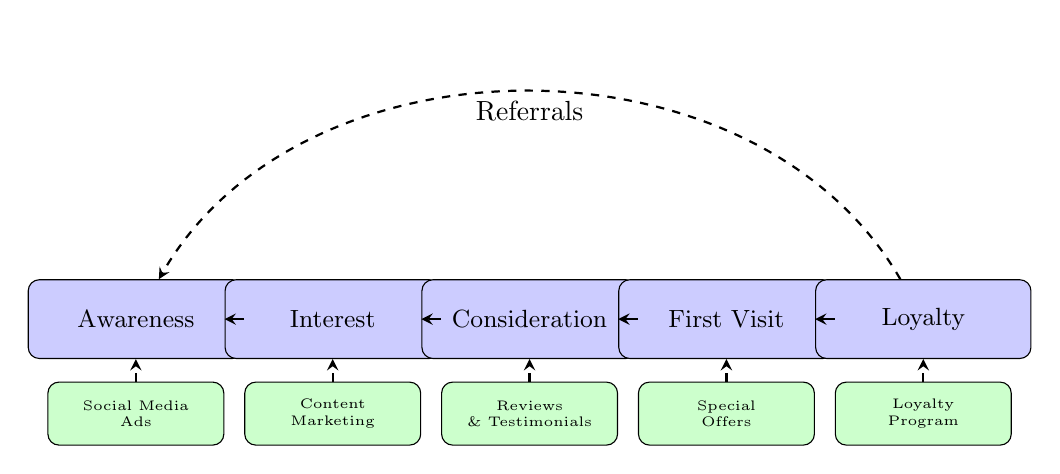
\begin{tikzpicture}[
    node distance=1.5cm,
    auto,
    stage/.style={rectangle, draw, fill=blue!20, text width=2.5cm, text centered, rounded corners, minimum height=1cm, font=\small},
    action/.style={rectangle, draw, fill=green!20, text width=2cm, text centered, rounded corners, minimum height=0.8cm, font=\tiny},
    arrow/.style={thick,->,>=stealth}
]
    % Customer journey stages
    \node [stage] (aware) {Awareness};
    \node [stage, right of=aware, xshift=1cm] (interest) {Interest};
    \node [stage, right of=interest, xshift=1cm] (consider) {Consideration};
    \node [stage, right of=consider, xshift=1cm] (visit) {First Visit};
    \node [stage, right of=visit, xshift=1cm] (loyal) {Loyalty};
    
    % Actions below each stage
    \node [action, below of=aware, yshift=0.3cm] (a1) {Social Media\\Ads};
    \node [action, below of=interest, yshift=0.3cm] (a2) {Content\\Marketing};
    \node [action, below of=consider, yshift=0.3cm] (a3) {Reviews\\\& Testimonials};
    \node [action, below of=visit, yshift=0.3cm] (a4) {Special\\Offers};
    \node [action, below of=loyal, yshift=0.3cm] (a5) {Loyalty\\Program};
    
    % Arrows between stages
    \draw [arrow] (aware) -- (interest);
    \draw [arrow] (interest) -- (consider);
    \draw [arrow] (consider) -- (visit);
    \draw [arrow] (visit) -- (loyal);
    
    % Feedback loop
    \draw [arrow, dashed, bend right=60] (loyal) to node [below] {Referrals} (aware);
    
    % Action connections
    \draw [arrow, dashed] (a1) -- (aware);
    \draw [arrow, dashed] (a2) -- (interest);
    \draw [arrow, dashed] (a3) -- (consider);
    \draw [arrow, dashed] (a4) -- (visit);
    \draw [arrow, dashed] (a5) -- (loyal);
\end{tikzpicture}
\caption{Customer Journey and Marketing Funnel}
\label{fig:customer_journey}
\end{figure}

\subsection{Marketing Objectives | 营销目标 | Marketingziele}

\begin{itemize}
    \item Build awareness in target market
    \item Attract new customers
    \item Encourage repeat visits
    \item Increase average check size
    \item Build community presence
    \item Generate positive word-of-mouth
\end{itemize}

\subsection{Target Audience | 目标受众 | Zielgruppe}

Defining your ideal customer:
\begin{itemize}
    \item Demographics (age, income, location)
    \item Psychographics (lifestyle, values, interests)
    \item Dining habits (frequency, occasions, preferences)
    \item Media consumption (where they get information)
\end{itemize}

\section{Marketing Channels | 营销渠道 | Marketingkanäle}

\subsection{Digital Marketing | 数字营销 | Digitales Marketing}

\subsubsection{Website}
\begin{itemize}
    \item Professional, mobile-responsive design
    \item Clear menu and pricing
    \item Online reservations
    \item Location and hours
    \item Contact information
    \item Photo gallery
    \item Blog or news section
    \item SEO optimization
\end{itemize}

\subsubsection{Social Media}

\textbf{Facebook}
\begin{itemize}
    \item Business page with complete information
    \item Regular posts (menu updates, events, behind-the-scenes)
    \item Photo and video content
    \item Event promotion
    \item Customer engagement
\end{itemize}

\textbf{Instagram}
\begin{itemize}
    \item High-quality food photography
    \item Stories for daily updates
    \item Reels for engaging content
    \item Hashtag strategy
    \item Influencer partnerships
\end{itemize}

\textbf{Other Platforms}
\begin{itemize}
    \item Twitter: News, engagement, customer service
    \item LinkedIn: B2B, corporate events
    \item TikTok: Creative, viral content
    \item Yelp, Google Business: Reviews and local search
\end{itemize}

\subsubsection{Email Marketing}
\begin{itemize}
    \item Newsletter with updates and specials
    \item Birthday and anniversary offers
    \item Event invitations
    \item Loyalty program communications
    \item Segmentation for targeted messaging
\end{itemize}

\subsubsection{Online Advertising}
\begin{itemize}
    \item Google Ads (local search)
    \item Social media advertising (Facebook, Instagram)
    \item Retargeting campaigns
    \item Local directory listings
\end{itemize}

\subsection{Traditional Marketing | 传统营销 | Traditionelles Marketing}

\subsubsection{Print Advertising}
\begin{itemize}
    \item Local newspapers and magazines
    \item Community publications
    \item Direct mail (postcards, flyers)
    \item Menus and brochures
\end{itemize}

\subsubsection{Outdoor Advertising}
\begin{itemize}
    \item Signage (exterior, directional)
    \item Billboards (if budget allows)
    \item Vehicle wraps
\end{itemize}

\subsection{Public Relations | 公共关系 | Öffentlichkeitsarbeit}

\subsubsection{Media Relations}
\begin{itemize}
    \item Press releases for openings, events, milestones
    \item Media kit (photos, story, contact info)
    \item Invite food critics and bloggers
    \item Build relationships with local media
\end{itemize}

\subsubsection{Community Involvement}
\begin{itemize}
    \item Sponsor local events
    \item Participate in community festivals
    \item Support local charities
    \item Partner with other businesses
\end{itemize}

\subsection{In-Restaurant Marketing | 餐厅内营销 | Marketing im Restaurant}

\begin{itemize}
    \item Table tents with specials
    \item Menu inserts
    \item Loyalty program promotion
    \item Event announcements
    \item Social media encouragement (check-ins, photos)
\end{itemize}

\section{Grand Opening Strategy | 开业策略 | Eröffnungsstrategie}

\subsection{Pre-Opening | 开业前 | Vor der Eröffnung}

\begin{itemize}
    \item \textbf{Soft opening}: Invite-only, friends, family, media
    \item \textbf{Staff training}: Practice service, refine operations
    \item \textbf{Media preview}: Invite food writers, bloggers
    \item \textbf{Social media}: Tease opening, build anticipation
\end{itemize}

\subsection{Grand Opening Events | 盛大开业活动 | Große Eröffnungsveranstaltungen}

\begin{itemize}
    \item \textbf{Ribbon cutting}: Local officials, media
    \item \textbf{Open house}: Community welcome
    \item \textbf{Special promotions}: Opening week deals
    \item \textbf{Press coverage}: Maximize visibility
\end{itemize}

\section{Customer Retention | 客户保留 | Kundenbindung}

\subsection{Loyalty Programs | 忠诚度计划 | Treueprogramme}

\begin{itemize}
    \item \textbf{Points system}: Earn points per visit or dollar spent
    \item \textbf{Punch cards}: Visit-based rewards
    \item \textbf{Membership tiers}: Different benefits levels
    \item \textbf{Digital apps}: Modern, convenient tracking
\end{itemize}

\subsection{Customer Relationship Management | 客户关系管理 | Kundenbeziehungsmanagement}

\begin{itemize}
    \item Collect customer information (with permission)
    \item Track visit frequency and preferences
    \item Personalized communications
    \item Special occasion recognition
    \item Feedback collection and response
\end{itemize}

\section{Special Events and Promotions | 特殊活动与促销 | Sonderveranstaltungen und Werbeaktionen}

\subsection{Regular Events | 定期活动 | Regelmäßige Veranstaltungen}

\begin{itemize}
    \item \textbf{Wine dinners}: Pairing events
    \item \textbf{Chef's table}: Special menu experiences
    \item \textbf{Live music}: Entertainment nights
    \item \textbf{Theme nights}: Special cuisines or concepts
    \item \textbf{Holiday events}: Valentine's, New Year's, etc.
\end{itemize}

\subsection{Promotions | 促销 | Werbeaktionen}

\begin{itemize}
    \item \textbf{Happy hour}: Discounted drinks and appetizers
    \item \textbf{Weekday specials}: Boost slower days
    \item \textbf{Seasonal menus}: Limited-time offerings
    \item \textbf{Group discounts}: Large party incentives
    \item \textbf{Gift card promotions}: Purchase incentives
\end{itemize}

\section{Online Reputation Management | 在线声誉管理 | Online-Reputationsmanagement}

\subsection{Review Platforms | 评论平台 | Bewertungsplattformen}

\begin{itemize}
    \item \textbf{Google Business}: Primary local search
    \item \textbf{Yelp}: Popular review site
    \item \textbf{OpenTable/Resy}: Reservation platforms
    \item \textbf{Facebook}: Reviews and recommendations
    \item \textbf{TripAdvisor}: Traveler reviews
\end{itemize}

\subsection{Managing Reviews | 管理评论 | Bewertungen verwalten}

\begin{itemize}
    \item \textbf{Monitor regularly}: Daily check of all platforms
    \item \textbf{Respond promptly}: Within 24-48 hours
    \item \textbf{Thank positive reviews}: Show appreciation
    \item \textbf{Address negative reviews}: Professional, solution-focused
    \item \textbf{Encourage reviews}: Ask satisfied customers
    \item \textbf{Never fake reviews}: Unethical and risky
\end{itemize}

\section{Marketing Budget | 营销预算 | Marketingbudget}

\subsection{Budget Allocation | 预算分配 | Budgetzuweisung}

Typical marketing budget: 3-5\% of sales
\begin{itemize}
    \item Digital marketing: 40-50\%
    \item Print and traditional: 20-30\%
    \item Events and promotions: 15-20\%
    \item Public relations: 10-15\%
    \item Contingency: 5-10\%
\end{itemize}

\subsection{ROI Measurement | ROI 衡量 | ROI-Messung}

Track marketing effectiveness:
\begin{itemize}
    \item Sales attributed to campaigns
    \item New customer acquisition
    \item Customer lifetime value
    \item Social media engagement
    \item Website traffic and conversions
    \item Review ratings and volume
\end{itemize}

\section{Partnerships and Collaborations | 合作伙伴关系与协作 | Partnerschaften und Kooperationen}

\subsection{Strategic Partnerships | 战略合作伙伴关系 | Strategische Partnerschaften}

\begin{itemize}
    \item \textbf{Local businesses}: Cross-promotion
    \item \textbf{Suppliers}: Feature in marketing
    \item \textbf{Event venues}: Catering partnerships
    \item \textbf{Tourism}: Visitor attraction partnerships
    \item \textbf{Influencers}: Social media collaborations
\end{itemize}

\section{Seasonal Marketing | 季节性营销 | Saisonales Marketing}

\subsection{Adapting to Seasons | 适应季节 | Anpassung an die Jahreszeiten}

\begin{itemize}
    \item \textbf{Menu changes}: Seasonal ingredients and dishes
    \item \textbf{Decor updates}: Reflect season or holidays
    \item \textbf{Special events}: Seasonal celebrations
    \item \textbf{Promotions}: Boost slower seasons
    \item \textbf{Marketing messages}: Align with season
\end{itemize}

\trilingualsection{Key Takeaways}{关键要点}{Wichtige Erkenntnisse}{}

\begin{itemize}
    \item Branding defines who you are; marketing communicates it
    \item Consistent brand identity builds recognition
    \item Digital marketing is essential in modern restaurant business
    \item Customer retention is as important as acquisition
    \item Online reputation requires active management
    \item Marketing budget should be planned and measured
    \item Partnerships can amplify marketing efforts
    \item Seasonal adaptation keeps marketing relevant
    \item Grand opening sets the tone for future success
\end{itemize}

With a strong brand and comprehensive marketing strategy, Sue and Owen were ready to welcome their first guests. The next chapter covers the critical opening day and the transition to ongoing operations.
